%!TEX root=./paper.tex
\section{Experiments}\label{sec:experiments}

In this section, we describe the experimental results of our model along with the parameters required to reproduce those results. We also describe baselines with which we compare our model and their parameters.

\subsection{Dataset Description}

We use the real-world traffic volumes of Dublin city streets collected using the SCATS (Sydney Coordinated Adaptive Traffic System)\cite{scats} system over a three-month period. The SCATS system is used in Dublin as an adaptive urban traffic management system that synchronizes traffic signals and optimizes traffic flow across the entire city.

The dataset consists of traffic volumes from the 825 sensors at all key intersections in Dublin city, sampled at a frequency of 1 hour during a time period of 3 months, from October 1, 2023, to December 31, 2023. The dataset contains the latitudinal and longitudinal geographical coordinates along with the timestamped total volume of traffic detected by each detector in the one-hour period.

The weather data used in conjunction with the traffic data is sourced from the official website of Met Éireann\cite{met_historical_data}, the state meteorological service of Ireland. The data contains hourly information on weather phenomena like air temperature, relative humidity, visibility, precipitation amount, etc., from three weather stations within the city of Dublin.

We also verify the model for the task (iii) on SUMO\cite{sumo} TAPASCologne scenario\cite{tapas}, which is a simulation configuration that describes the traffic dynamics of Cologne city in Germany for a day. The scenario is publicly available on the official SUMO website and was created using mobility demand data based on information about the traveling habits of citizens and information about the infrastructure of the area they live in. Since this testing is manual, we run a limited number of tests, where we change an edge and process the simulation based on the default minimal travel time routing before and after the change and observe the deviation between the simulation and our results.

\begin{figure}[htbp]
  \centering
  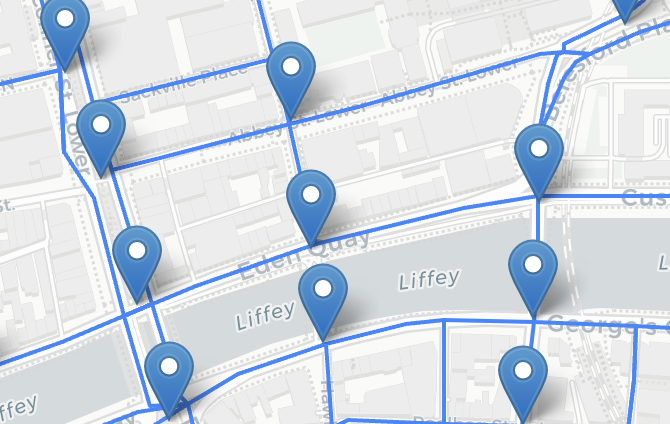
\includegraphics[width=0.5\textwidth]{dataset.png}
  \caption{Snapshot of sensor locations plotted along with road network from Overpass API}
  \label{fig:dataset}
\end{figure}


\subsection{Model Parameters}

For all experiments, we set hyperparameters $T = 3$, which is the number of consecutive timesteps to consider for prediction and imputation tasks. For all tasks, we optimize the model input by assuming the locality of traffic within such a timespan and that any changes to a particular node are only dependent on nodes "close" to it. During training, we train on sub-graphs consisting of the node clusters instead of the entire graph all at once. Specifically, a subgraph is generated by choosing a node $u$ at random and then selecting all nodes that are at a distance less than $\sigma$ to it, specifically for $G(V, E)$, $G_{\text{sub}} = G\{v \in V \; | \; \text{dist}(u, v) < \sigma\}$. For our experiments, we set $\sigma$ as $2.5\ km$, which is a reasonable expectation as clusters usually contain 20 to 30 nodes within this range.

After sampling, as stated before, we use an 80-20 test-train split, i.e., the model is trained on 80\% of the samples, and then performance is verified on new unseen data that comprises 20\% of the samples. The data is then modified based on the task at hand. For imputation, we followed MCAR (Missing Completely at Random) distribution and randomly masked values both spatially and temporally, following a parameter defined as the miss rate, we tested our model on miss rates of 10\%, 20\%, 30\%, and 40\%. For prediction, we use the full data of three timesteps to predict the fourth step by basically masking the values along the last timestep dimension. For the re-assignment task, i.e., task (iii), we only consider one timestep and re-assign values for that same timestep but with modified spatial geometry.

\subsection{Baselines}

We compare our \name\ model with a number of different existing approaches across different domains, including different mathematical analysis and deep learning techniques used popularly for these tasks.

One of the simplest approaches for imputation is \textit{KNN}. Similarly, for prediction, \textit{ARIMA}\cite{arima} stands for AutoRegressive Integrated Moving Average is used. Matrix factorization methods like \textit{TRMF}\cite{trmf} (Temporal Regularized Matrix Factorization) use latent factors for predictions, and its modification \textit{BTRMF}\cite{btrmf} (Bayesian Temporal Regularized Matrix Factorization) extends TRMF with a Bayesian framework. For both these methods, we use rank $= 10$, $1000$ burn-in iterations, and $200$ Gibbs iterations.

\textit{LRTC-TNN}\cite{lrtc} (Low-Rank Tensor Completion with Truncated Nuclear Norm) is a method for tensor completion. It uses parameters $\rho = 1e-5$, $\theta = 0.25$, and $\epsilon = 1e-4$. \textit{BGCP} (Bayesian Gaussian Process Factorization) is another method that utilizes Bayesian inference. For BGCP, we use similar burn-in and Gibbs iterations and set rank $= 30$. It is worth noting that these model baselines are only applicable to task (i) and task (ii) and not to task (iii) since they were not built with that task as a consideration.

Finally, there are deep learning methods that we used. For imputation, we employed the \textit{Denoising AutoEncoder} (DAE)\cite{dae} model, which is effective in learning meaningful representations of the data while handling missing values. For prediction tasks, we utilized an \textit{LSTM}\cite{lstm} (Long Short-Term Memory) model as LSTM networks are well-suited for capturing temporal dependencies in sequential data.

\subsection{Evaluation metrics}

In order to evaluate the performance of the different methods and compare them, we use RMSE (Root Mean Squared Error) and MAPE (Mean Absolute Percentage Error). These metrics are defined as:


\[
\text{RMSE} = \sqrt{\frac{1}{n} \sum_{i=1}^{n} (y_i - \hat{y}_i)^2}
\]

\[
\text{MAPE} = \frac{1}{n} \sum_{i=1}^{n} \left| \frac{y_i - \hat{y}_i}{y_i} \right| \times 100\%
\]

where \( y_i \) represents the true value, \( \hat{y}_i \) represents the predicted value, and \( n \) is the number of samples.